Nesta seção é apresentado a simulação do escoamento
de \textit{Poiseuille} na metade do domínio. Dessa forma,
a condição de contorno de superfície livre de escorregamento
é necessária no eixo de simetria.
A \ref{half poiseuille} apresenta esquematicamente este escoamento com o
eixo de simetria especificado e
o perfil do campo de velocidade esperado.

\begin{figure}[H]
\begin{center}
\begin{tikzpicture}[scale=1.2]
 \draw [pattern=north east lines] (0,1) -- (0,1.1) -- (5,1.1) -- (5,1) -- cycle;
 \draw [dashed] (-0.3,0.0) to (5.3,0.0);

 \draw [->,thick] (-2,-0.1)--(-2,1.5) node[left] {$y$};
 \draw [->,thick] (-2.1,0)--(-0.5,0) node[below] {$x$};

 \draw [->,thick] (5.4,0.0)--(6.1,0.0);
 \node [draw=none] at (7.1,0.0) {$simetria$};
 
 \draw [dotted] (2.5,0.0) to (2.5,1.0);
 \draw  (2.8,0.0) to [bend right=20] (2.5,1.0);
 
 \draw [->,thick] (2.5,0.0) to (2.8,0.0);
 \draw [->,thick] (2.5,0.3) to (2.78,0.3);
 \draw [->,thick] (2.5,0.6) to (2.71,0.6);
 \draw [->,thick] (2.5,0.85) to (2.6,0.85);
\end{tikzpicture}
\end{center}
\caption{Escoamento de Poiseuille em Meio Domínio}
\label{half poiseuille}
\end{figure}

\noindent
O perfil de velocidade que este escoamento adquire 
é dado pela equação abaixo:

\begin{equation}
 u = u_{max} \big[ 1 - \frac{y^{2}}{L^{2}} \big]
\end{equation}


\medskip
\noindent
onde $u_{max}$ é a velocidade máxima e seu valor é
$u_{max} = 1.5$, $L$ é a largura não dimensional
entre a placa e o eixo de simetria, seu valor é $L = 1$
e $y$ é a distância entre a placas e o eixo de simetria,
a mesma varia entre $y = \big[ 0,1 \big]$.
O domínio foi discretizado utilizando uma malha 
triangular linear com 3835 nós e 7299 elementos. 

\medskip
\noindent
As condições de contorno utilizadas foram:

\begin{itemize}
     \item \textit{condição de entrada}:
      a componente normal da velocidade $v=0$ enquanto a componente tangencial da velocidade é $u = 1$.                 
      A função de corrente também é especificada e seu valor é definido segundo a equação da continuidade  
      para um fluido incompressível. Dessa forma, seu valor será $\psi = y$.

     \item \textit{condição de não escorregamento}: esta condição é utilizada na placa superior, 
      onde todas as componentes da velocidade são especificadas    
      com os valores $u=0$ e $v=0$.                       
      A função de corrente também é espeficado com o valor $\psi=1$.               
      
     \item \textit{condição de saída}: O valor da função de corrente é especificado $\psi=y$. As derivadas das 
     componentes tangencial e normal da velocidade possuem o 
     valor nulo, isto é,
      $\partial u/\partial n = 0$ e
      $\partial v/\partial n = 0$ respectivamente.   

     \item \textit{condição de livre escorregamento}: esta condição é utilizada no eixo de simetria.
      A componente normal da velocidade e a função de corrente possuem seus valores especificados,
      tais como $v=0$ e $\psi=0$ respectivamente. A derivada da componente tangencial da velocidade
      possuei o valor nulo $\partial u/\partial n = 0$.
\end{itemize}

\medskip
A \ref{velocidade half poiseuille} apresenta a evolução 
do perfil de velocidade no tempo quando o $Re=100$, além do comparativo
entre a solução numérica e a solução analítica no estado permanente do
problema proposto. É possível observar um pequeno desvio entre a solução numérica
e a solução analítica próximo ao eixo de simetria. 

\begin{figure}[H]
     \centering
     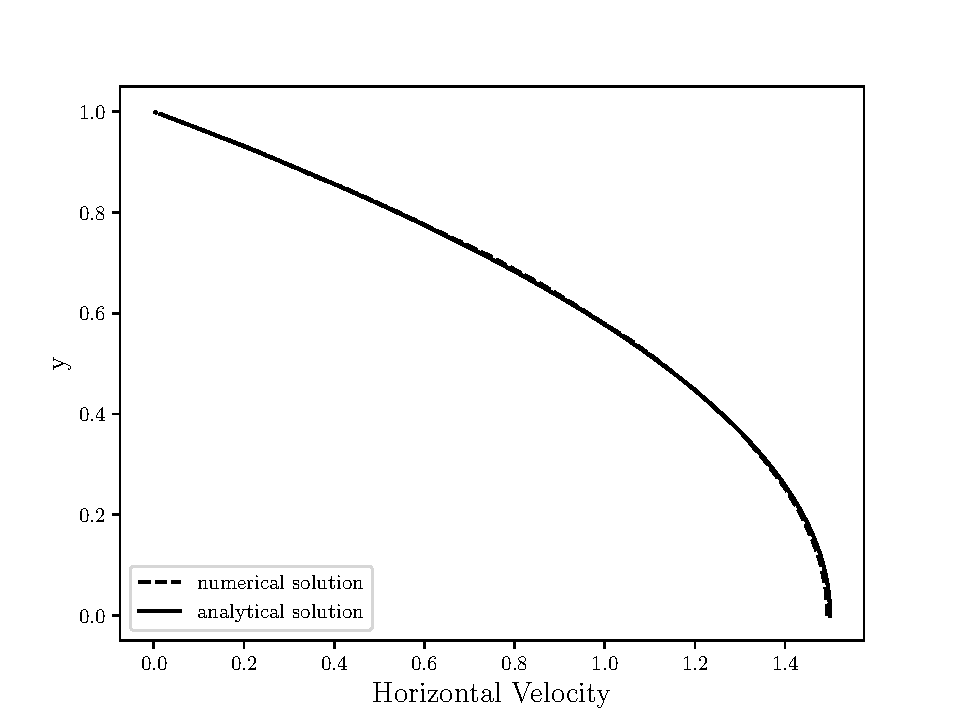
\includegraphics[scale=1]{./02_chaps/cap_validation/figure/half_poiseuille_velocity.pdf}\\
     \medskip
     \caption{Evolução do perfil de velocidade no tempo para $Re=100$ e
     a comparação da solução numérica com a solução analítica para o Escoamento de Poiseuille em Meio Domínio.}
     \label{velocidade half poiseuille}
\end{figure}

\newpage
